\documentclass[journal,12pt,twocolumn]{IEEEtran}

\usepackage[utf8]{inputenc}
\usepackage{kvmap}
\usepackage{graphics} 

\usepackage{setspace}
\usepackage{gensymb}

\singlespacing

\usepackage{amsthm}

\usepackage{mathrsfs}
\usepackage{txfonts}
\usepackage{stfloats}
\usepackage{bm}
\usepackage{cite}
\usepackage{cases}
\usepackage{subfig}

\usepackage{longtable}
\usepackage{multirow}

\usepackage{enumitem}
\usepackage{mathtools}
\usepackage{steinmetz}
\usepackage{tikz}
\usepackage{circuitikz}
\usepackage{verbatim}
\usepackage{tfrupee}
\usepackage[breaklinks=true]{hyperref}
\usepackage{graphicx}
\usepackage{tkz-euclide}
\usepackage{float}

\usetikzlibrary{calc,math}
\usepackage{listings}
    \usepackage{color}                                            %%
    \usepackage{array}                                            %%
    \usepackage{longtable}                                        %%
    \usepackage{calc}                                             %%
    \usepackage{multirow}                                         %%
    \usepackage{hhline}                                           %%
    \usepackage{ifthen}                                           %%
    \usepackage{lscape}     
\usepackage{multicol}
\usepackage{chngcntr}

\DeclareMathOperator*{\Res}{Res}

\renewcommand\thesection{\arabic{section}}
\renewcommand\thesubsection{\thesection.\arabic{subsection}}
\renewcommand\thesubsubsection{\thesubsection.\arabic{subsubsection}}

\renewcommand\thesectiondis{\arabic{section}}
\renewcommand\thesubsectiondis{\thesectiondis.\arabic{subsection}}
\renewcommand\thesubsubsectiondis{\thesubsectiondis.\arabic{subsubsection}}

\hyphenation{op-tical net-works semi-conduc-tor}
\def\inputGnumericTable{}                                 %%

\lstset{
%language=C,
frame=single, 
breaklines=true,
columns=fullflexible
}
\begin{document}

\newtheorem{theorem}{Theorem}[section]
\newtheorem{problem}{Problem}
\newtheorem{proposition}{Proposition}[section]
\newtheorem{lemma}{Lemma}[section]
\newtheorem{corollary}[theorem]{Corollary}
\newtheorem{example}{Example}[section]
\newtheorem{definition}[problem]{Definition}

\newcommand{\BEQA}{\begin{eqnarray}}
\newcommand{\EEQA}{\end{eqnarray}}
\newcommand{\define}{\stackrel{\triangle}{=}}
\newcommand\hlight[1]{\tikz[overlay, remember picture,baseline=-\the\dimexpr\fontdimen22\textfont2\relax]\node[rectangle,fill=blue!50,rounded corners,fill opacity = 0.2,draw,thick,text opacity =1] {$#1$};}
\bibliographystyle{IEEEtran}
\providecommand{\mbf}{\mathbf}
\providecommand{\pr}[1]{\ensuremath{\Pr\left(#1\right)}}
\providecommand{\qfunc}[1]{\ensuremath{Q\left(#1\right)}}
\providecommand{\sbrak}[1]{\ensuremath{{}\left[#1\right]}}
\providecommand{\lsbrak}[1]{\ensuremath{{}\left[#1\right.}}
\providecommand{\rsbrak}[1]{\ensuremath{{}\left.#1\right]}}
\providecommand{\brak}[1]{\ensuremath{\left(#1\right)}}
\providecommand{\lbrak}[1]{\ensuremath{\left(#1\right.}}
\providecommand{\rbrak}[1]{\ensuremath{\left.#1\right)}}
\providecommand{\cbrak}[1]{\ensuremath{\left\{#1\right\}}}
\providecommand{\lcbrak}[1]{\ensuremath{\left\{#1\right.}}
\providecommand{\rcbrak}[1]{\ensuremath{\left.#1\right\}}}
\theoremstyle{remark}
\newtheorem{rem}{Remark}
\newcommand{\sgn}{\mathop{\mathrm{sgn}}}
\providecommand{\abs}[1]{\left\vert#1\right\vert}
\providecommand{\res}[1]{\Res\displaylimits_{#1}} 
\providecommand{\norm}[1]{$\left\lVert#1\right\rVert$}
%\providecommand{\norm}[1]{\lVert#1\rVert}
\providecommand{\mtx}[1]{\mathbf{#1}}
\providecommand{\mean}[1]{E\left[ #1 \right]}
\providecommand{\fourier}{\overset{\mathcal{F}}{ \rightleftharpoons}}
%\providecommand{\hilbert}{\overset{\mathcal{H}}{ \rightleftharpoons}}
\providecommand{\system}{\overset{\mathcal{H}}{ \longleftrightarrow}}
	%\newcommand{\solution}[2]{\textbf{Solution:}{#1}}
\newcommand{\solution}{\noindent \textbf{Solution: }}
\newcommand{\cosec}{\,\text{cosec}\,}
\providecommand{\dec}[2]{\ensuremath{\overset{#1}{\underset{#2}{\gtrless}}}}
\newcommand{\myvec}[1]{\ensuremath{\begin{pmatrix}#1\end{pmatrix}}}
\newcommand{\mydet}[1]{\ensuremath{\begin{vmatrix}#1\end{vmatrix}}}
\numberwithin{equation}{subsection}
\makeatletter
\@addtoreset{figure}{problem}
\makeatother
\let\StandardTheFigure\thefigure
\let\vec\mathbf
\renewcommand{\thefigure}{\theproblem}
\def\putbox#1#2#3{\makebox[0in][l]{\makebox[#1][l]{}\raisebox{\baselineskip}[0in][0in]{\raisebox{#2}[0in][0in]{#3}}}}
     \def\rightbox#1{\makebox[0in][r]{#1}}
     \def\centbox#1{\makebox[0in]{#1}}
     \def\topbox#1{\raisebox{-\baselineskip}[0in][0in]{#1}}
     \def\midbox#1{\raisebox{-0.5\baselineskip}[0in][0in]{#1}}
\vspace{3cm}
\title{\textbf{Matrices Assignment - Circle} }
\author{Dukkipati Vijay Sai}
\maketitle
\newpage
\bigskip
\renewcommand{\thefigure}{\theenumi}
\renewcommand{\thetable}{\theenumi}
Get Python code for the figure from 
\begin{lstlisting}
https://github.com/dukkipativijay/Fwciith2022/tree/main/Assignment%201/Codes/src
\end{lstlisting}
Get LaTex code from
\begin{lstlisting}
https://github.com/dukkipativijay/Fwciith2022/tree/main/Assignment%201%20-%20Assembly/Codes
\end{lstlisting}
%
\section{Question}
\centering
\textbf{\textit{Class 10, Exercise 11.2, Q(1)}}\\
\vspace{0.25cm}
\raggedright
\textbf{Draw a circle of radius 6cm. From a point 10cm away from the centre, construct the pair of tangents to the circle and measure their lengths.} \\
\raggedright
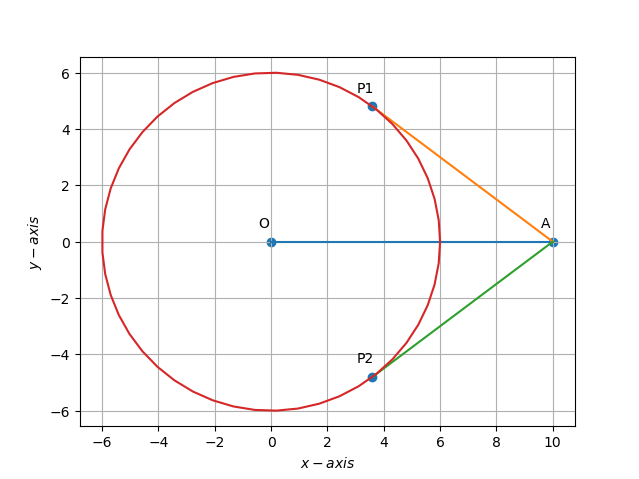
\includegraphics[width=0.5\textwidth]{circle fig.png}
Figure 1 - Circle with Tangents $AP_1$, $AP_2$

\section{Construction}
\vspace{0.25cm}
\raggedright
A circle with centre O, radius 6cm and the tangents $AP_1$, $AP_2$ from a point A located 10cm away from the centre were constructed using Python, with the following parameters shown in the table below.\\
\begin{tabular}{|c|c|c|}
\hline
\textbf{Symbol} & \textbf{Value} & \textbf{Description}\\
\hline
O & $\myvec{0\\0}$ & Center \\
\hline
r & 6cm & Radius \\
\hline
d & 10cm & Distance between O and A\\
\hline
$e_1$ & $\myvec{1\\0}$ & Unit Vector along X-Axis\\
\hline
A & d x $e_1$ & Point A \\
\hline
$\theta$ & $\angle P_1OA$ & Angle $P_1$OA\\
\hline
$P_1$ & $r \myvec{cos\theta\\sin\theta}$ & Point of Contact $P_1$\\
\hline
$P_2$ & $r \myvec{cos\theta\\-sin\theta}$ & Point of Contact $P_2$\\
\hline
\end{tabular}\\
\vspace{0.2cm}
\centerline{Table 1: Parameters Table}
\section{Solution}

Consider the circle of radius 6cm whose center is at origin and point A at a distance of 10cm away from the center.\\

Two tangents can be drawn from point A on to the circle and let the point of contacts be $P_1$ and $P_2$.\\

\vspace{0.25cm}

The point of intersection of line\\
\centering
\begin{align}
L : \vec{x} = \vec{q} + \mu \vec{m}  \hspace{0.4cm} \mu \epsilon \mathbb{R}
\end{align} 
\raggedright
With the conic section,\\
\centering
\begin{align}
\vec{x}^T \vec{V}\vec{x} + 2 \vec{u}^T \vec{x} + f = 0
\label{eq2}
\end{align}
\raggedright
is given by\\
\centering
\begin{align}
\vec{x}_i = \vec{q} + \mu_i \vec{m}
\label{eq3}
\end{align}
\raggedright
Where,\\
$\mu_i = \frac{1}{\vec{m^T Vm}}(-\vec{m^T(Vq+u)}$ \\ 
\begin{align}
\pm \sqrt{[\vec{m^T(Vq+u})]^2 - (\vec{q}^T \vec{Vq} + 2 \vec{u^T q} + f) (\vec{m^T Vm})} )
\label{eq4}
\end{align}
\raggedright
If the line L touches the conic at exactly one point,the conic intercept has exactly one root. Hence, \\
\centering
\begin{align}
[\vec{m^T(Vqu})]^2 - (\vec{m^T Vm}) (\vec{q}^T \vec{Vq} + 2 \vec{u^T q} + f)  = 0
\label{eq5}
\end{align}
\raggedright
The equation of our circle is,\\
\centering 
\begin{align}
x^2 + y^2 = 36
\label{eq6}
\end{align}
\raggedright
Comparing it with the General Equation of a circle,\\
\centering
\begin{align}
Ax^2 + Bxy + Cy^2 + Fx + Gy + f = 0
\end{align}
\raggedright
We Have,\\
\vspace{0.25cm}
A = 1, B = 0, C = 1, F = 0, G = 0, f = -36\\
\vspace{0.25cm}
We Know That,\\
\vspace{0.25cm}
\centering
$ V = \myvec{A&\frac{B}{2}\\\\\frac{B}{2}&C} \hspace{2cm} u = \myvec{\frac{F}{2}\\\\\frac{G}{2}} $\\
\vspace{0.25cm}
\raggedright
So we get,\\
\vspace{0.25cm}
\centering
$ V = \myvec{1&0\\0&1} \hspace{2.2cm} u = \myvec{0\\0} $ \\
\vspace{0.25cm}
\raggedright
Hence, the Eq.\eqref{eq6} of our circle can be written in the form of Conic Eq.\eqref{eq2} as,\\
\centering
\begin{align}
\vec{x^T} \myvec{1&0\\0&1}\vec{x} + 2 \myvec{0&0} \vec{x} - 36 = 0
\label{eq8}
\end{align} 
\raggedright
Let us consider the direction vector of \textbf{L} as m,\\
\centering
\begin{align}
\vec{m} = \myvec{1\\ \lambda}
\label{eq9}
\end{align}
\raggedright
and \textbf{q} be the point A,\\
\centering
\begin{align}
\vec{q} = \myvec{10\\0}
\label{eq10}
\end{align}
\vspace{0.5cm}
\raggedright
Substituting Eq.\eqref{eq8}, \eqref{eq10} and \eqref{eq10} in Eq.\eqref{eq5}, we get\\
\vspace{0.5cm}
\centering
$ [\vec{m^T(Iq})]^2 - (\vec{m^T Im}) (\vec{q}^T \vec{Iq} + (-36)  = 0$\\
\vspace{0.25cm}
$ [ \myvec{1& \lambda} \myvec{10\\0} ]^2 - ( \myvec{1&\lambda}\myvec{1\\\lambda} ) (\myvec{10&0} \myvec{10\\0} - 36 ) = 0$ \\
\hspace{8cm} \\ 
\vspace{0.25cm}
$ (10)^2 - ( 1 + \lambda^2 ) (100 - 36 ) = 0$\\
\vspace{0.25cm}
$ 100 - ( 1 + \lambda^2 ) ( 64 ) = 0 $\\
\vspace{0.25cm}
$ (1 + \lambda^2 ) (64 ) = 100 $\\
\vspace{0.25cm}
$ 1 + \lambda^2 = \frac{100}{64} $\\
\vspace{0.25cm}
$ \lambda^2 = \frac{36}{64} $ \\
\vspace{0.25cm}
$ \lambda = \pm \frac{6}{8} $ \\
\vspace{0.25cm}
$ \therefore \lambda = \pm \frac{3}{4} = \pm 0.75 $ \\ 
\vspace{0.25cm}
\raggedright
Hence,\\
\vspace{0.25cm}
\centering
$ m = \myvec{1 \\ \pm \frac{3}{4}} $ \\
\vspace{0.25cm}
\raggedright
From Eq.\eqref{eq4} and \eqref{eq5}\\
\vspace{0.25cm}
\centering
$ \mu_i = \frac{1}{\vec{m^T Vm}} ( - \vec{m^T (Vq + u)})$\\
\vspace{0.25cm}
$ \mu_i = \frac{1}{\myvec{1 & \frac{3}{4}} \vec{I} \myvec{1\\\frac{3}{4}}} ( - \myvec{1&\frac{3}{4}} ( \vec{I}\myvec{10\\0})$\\ 
\vspace{0.25cm}
$ \mu_i = \frac{1}{1 + \frac{9}{16}} ( - (10 + 0) )$\\
\vspace{0.25cm}
$ \mu_i = \frac{-10}{\frac{25}{16}}$\\
\vspace{0.25cm}
$ \mu_i = \frac{-32}{5} $ \\
\vspace{0.25cm}
$ \mu_i = -6.4 $\\
\vspace{0.4cm}
\raggedright
Now Eq.\eqref{eq3} becomes,\\
\vspace{0.25cm}
\centering
$ \myvec{x \\ y} = \myvec{10\\0} + (-6.4)  \myvec{1 \\ \pm 0.75} $ \\
\vspace{0.25cm}
$ \myvec{x \\y } = \myvec{10\\0} + \myvec{-6.4 \\ \mp 4.8} $ \\
\vspace{0.25cm}
$ \myvec{x \\y } = \myvec{3.6\\\mp 4.8} $ \\
\vspace{0.25cm}
$ \myvec{x \\y } = \myvec{3.6\\ 4.8} or \myvec{x \\y } = \myvec{3.6\\ -4.8} $ \\
\vspace{0.25cm} 
\raggedright
Therefore,\\
\vspace{0.25cm}
\centering
$ P_1 = \myvec{3.6\\ 4.8}$ \\
\vspace{0.25cm}
$P_2 = \myvec{3.6\\ -4.8} $ \\
\vspace{0.4cm}
\raggedright
Now,\\
\vspace{0.25cm}
Length of Tangent 1 = $ \| \vec{P_1} - \vec{A} \| $\\
\vspace{0.25cm}
\centering
$ = \| \myvec{3.6\\4.8} - \myvec{8\\0} \| $\\
\vspace{0.25cm}
$ = \| \myvec{-4.4\\4.8} \| $ \\
\vspace{0.25cm}
$ = 8cm $\\
\vspace{0.25cm}
\raggedright
Similarly,\\
\vspace{0.25cm}
Length of Tangent 2 = $ \| \vec{P_2} - \vec{A} \| $\\
\vspace{0.25cm}
\centering
$ = \| \myvec{3.6\\-4.8} - \myvec{8\\0} \| $\\
\vspace{0.25cm}
$ = \| \myvec{-4.4\\-4.8} \| $ \\
\vspace{0.25cm}
$ = 8cm $\\
\end{document}
Footer